\begin{wrapfigure}{r}{0pt}
  \centering
  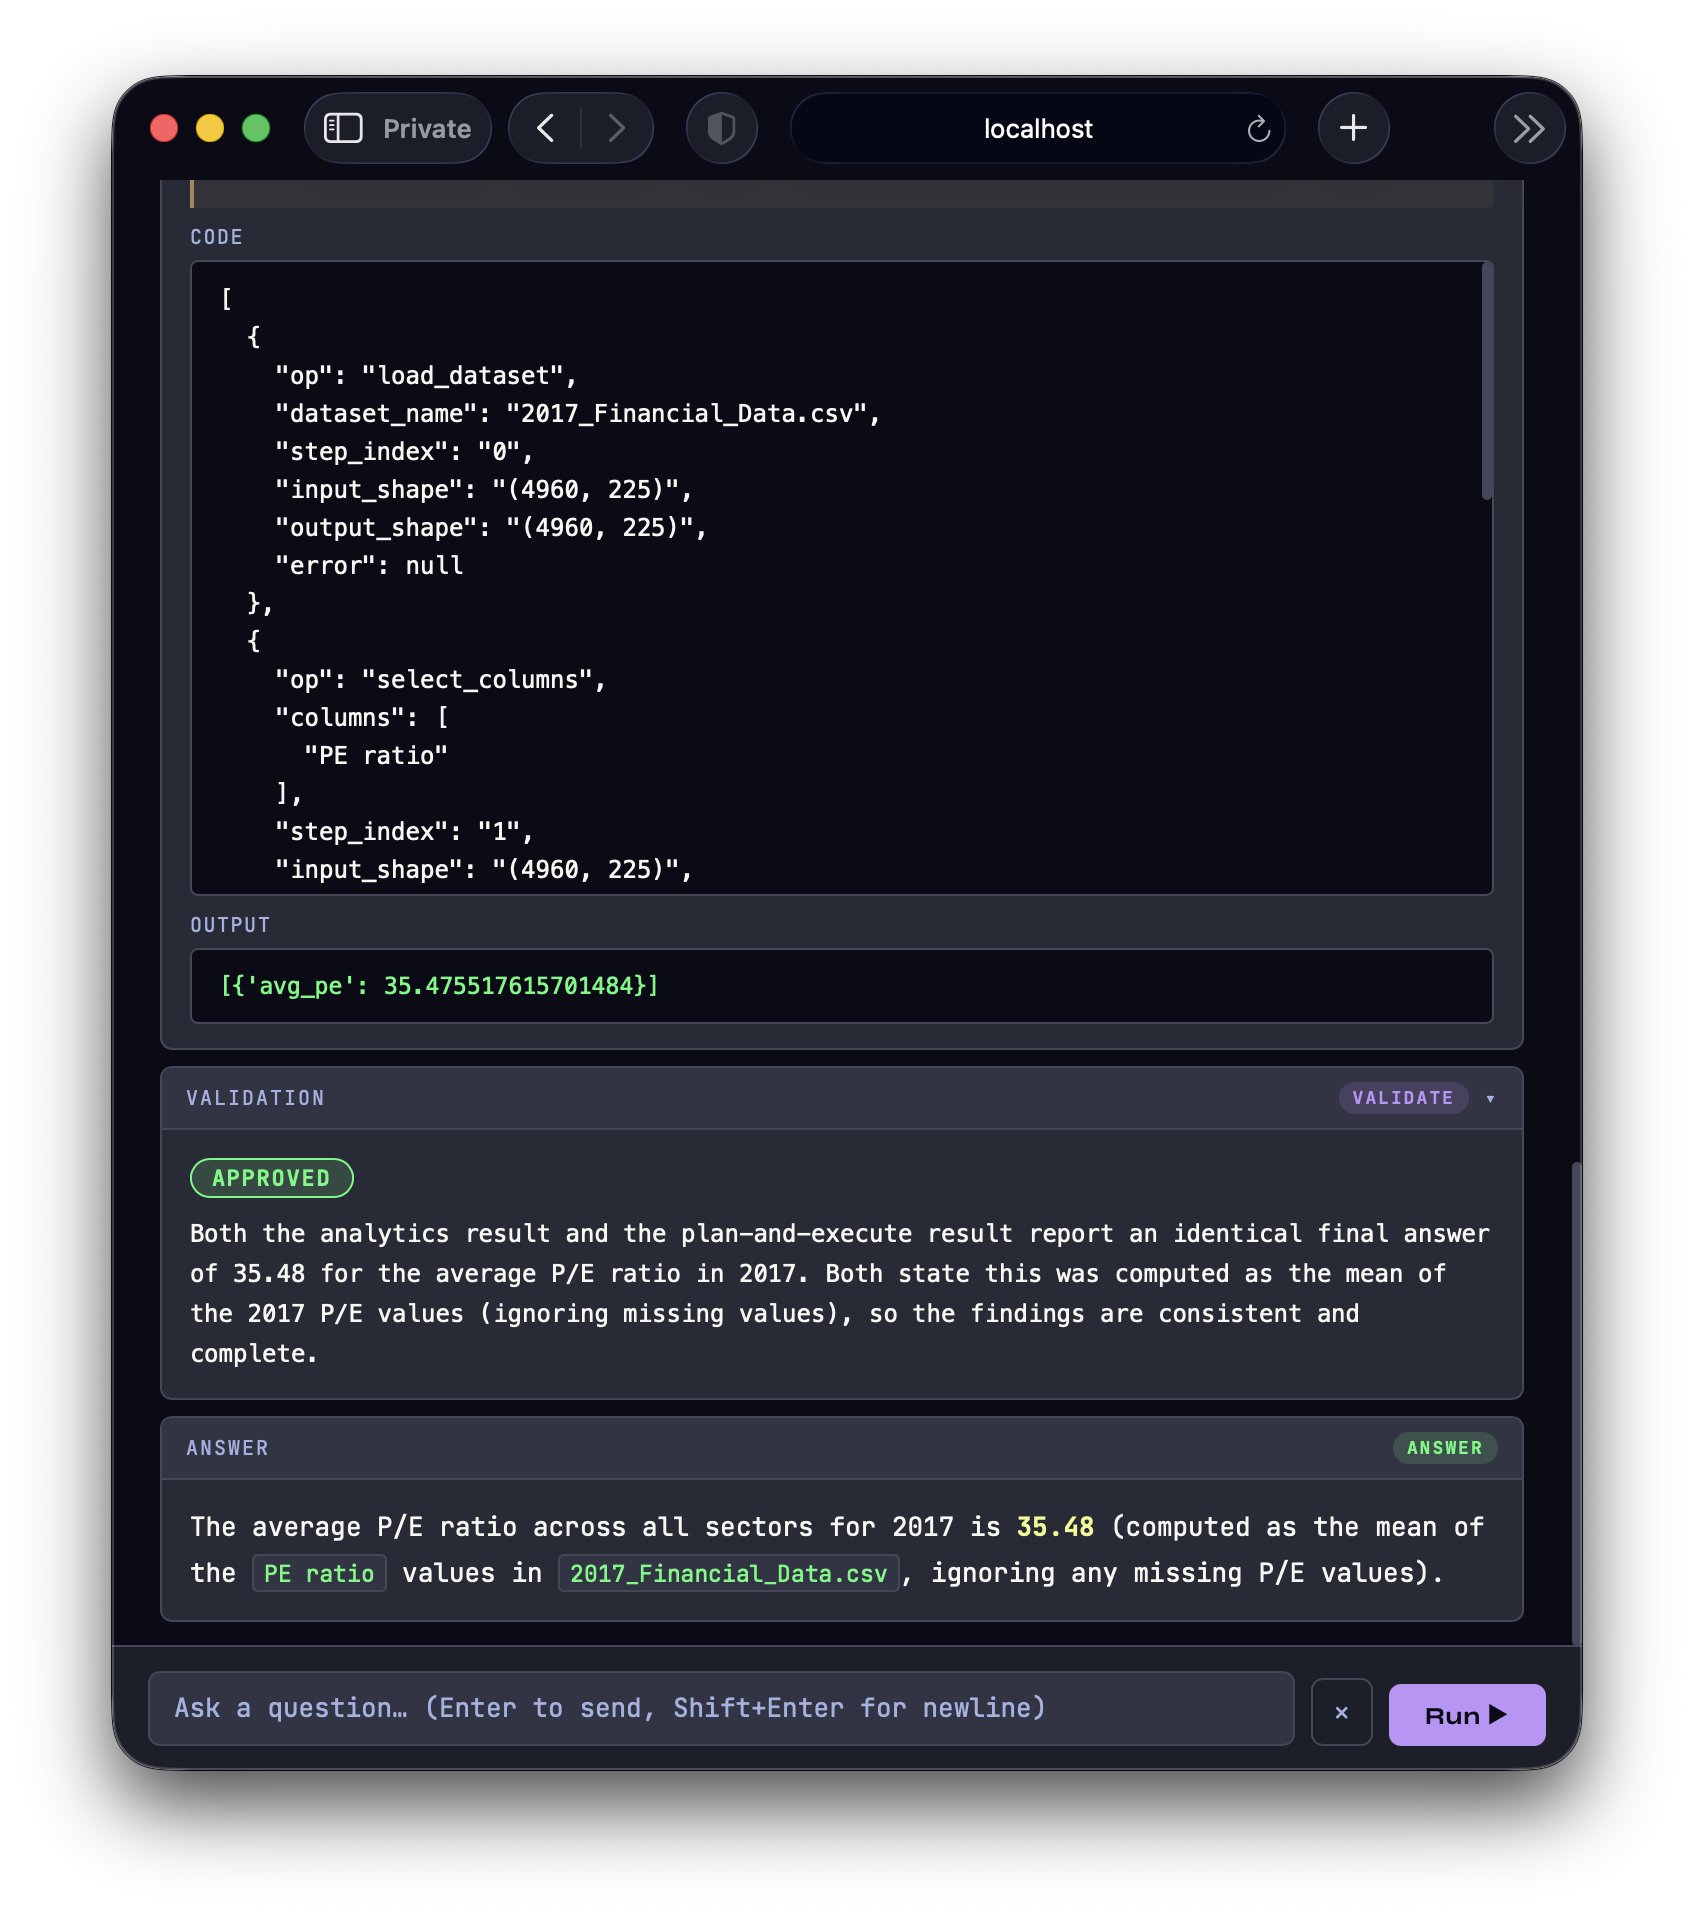
\includegraphics[width=0.4\textwidth]{graphics/ui-what-is-the-average-p-e-ratio-across-all-sectors-for-2017.png}
  \caption{UI Screenshot}
\end{wrapfigure}

This example demonstrates a successful execution in which the validator approves the result on the first attempt. No retry requests are issued because the independent solution paths agree on the final answer.

From the input specification, it identifies a single dataset, \texttt{2017\_Financial\_Data.csv}. The task is interpreted as computing the overall mean of the \texttt{PE ratio} column across all rows in the dataset. The agent explicitly notes that missing values should be ignored when computing the mean.

\subsect{Analytics Agent Execution}

The analytics agent performs a direct computation using Python. It:

\begin{enumerate}
  \item Loads \texttt{2017\_Financial\_Data.csv}.
  \item Converts the \texttt{PE ratio} column to numeric values.
  \item Computes the mean using \texttt{mean(skipna=True)}.
  \item Produces the result:
    \[
      35.475517615701484
    \]
\end{enumerate}

The agent then rounds the value for presentation and generates the answer:

\begin{quote}
  The average P/E ratio across all sectors for 2017 is \textbf{35.48}.
\end{quote}

A follow-up analytics reasoning step verifies that no additional computation is required because the requested quantity is a single global average.

\subsect{Plan-and-Execute Agent}

In parallel, the planning agent constructs an explicit execution plan. The plan consists of four operations:

\begin{enumerate}
  \item \texttt{load\_dataset} on \texttt{2017\_Financial\_Data.csv}.
  \item \texttt{select\_columns} to retain only \texttt{PE ratio}.
  \item \texttt{group\_aggregate} with an empty grouping key, computing the mean of \texttt{PE ratio}.
  \item \texttt{display} the resulting single-row output.
\end{enumerate}

The planner therefore reaches the same numerical result and produces the answer:

\begin{quote}
  The average P/E ratio across all sectors for 2017 is 35.48.
\end{quote}

\subsect{Validation Agent}

The validation agent compares the outputs of the analytics pipeline and the plan-and-execute pipeline.

It verifies that:

\begin{itemize}
  \item Both methods compute the mean of the 2017 \texttt{PE ratio} values.
  \item Both explicitly ignore missing values.
  \item Both produce the identical final answer, \(35.48\).
\end{itemize}

The validator records the verdict:

\begin{quote}
  \texttt{approved}
\end{quote}

The validator's reasoning states that the findings are consistent and complete because the independently generated solutions agree exactly.

\subsect{Retry Analysis}

No retry cycle occurs in this example.

The validation output contains:

\begin{itemize}
  \item Verdict: \texttt{approved}
  \item Feedback: \texttt{null}
\end{itemize}

Because no discrepancies, execution errors, or inconsistencies are detected, the validator does not request additional work from either agent. The workflow therefore terminates after the initial validation pass.

\subsect{Final Outcome}

The system successfully answers the question on the first attempt. Agreement between the analytics agent and the plan-and-execute agent allows the validator to approve the result immediately, eliminating the need for any retry requests or corrective actions.
